\documentclass[aspectratio=169]{beamer}

% ---- Packages ----------------------------------------------------------------
\usepackage[T1]{fontenc}
\usepackage[utf8]{inputenc}
\usepackage{amsmath,amssymb}
\usepackage{booktabs}
\usepackage{tikz}
\usetikzlibrary{arrows.meta,positioning,shapes.geometric,backgrounds,fit}
\usepackage{xcolor}
\usepackage{graphicx}
\usepackage{hyperref}
\usepackage{microtype}

% ---- Colour palette ----------------------------------------------------------
\definecolor{mqblue}{RGB}{0,73,135}       % deep institute blue
\definecolor{mqgold}{RGB}{200,155,40}     % warm gold accent
\definecolor{mqlight}{RGB}{220,232,245}   % very light blue tint
\definecolor{mqmid}{RGB}{90,140,195}      % mid blue for accents
\definecolor{mqgray}{RGB}{80,80,80}       % body text gray
\definecolor{mqalert}{RGB}{180,40,40}     % red for emphasis

% ---- Beamer theme ------------------------------------------------------------
\usetheme{default}
\usecolortheme{default}
\usefonttheme{professionalfonts}

\setbeamercolor{frametitle}{fg=white,bg=mqblue}
\setbeamercolor{title}{fg=white}
\setbeamercolor{subtitle}{fg=mqgold}
\setbeamercolor{author}{fg=mqlight}
\setbeamercolor{date}{fg=mqlight}
\setbeamercolor{normal text}{fg=mqgray}
\setbeamercolor{structure}{fg=mqblue}
\setbeamercolor{alerted text}{fg=mqalert}
\setbeamercolor{block title}{fg=white,bg=mqblue}
\setbeamercolor{block body}{fg=mqgray,bg=mqlight}
\setbeamercolor{itemize item}{fg=mqgold}
\setbeamercolor{itemize subitem}{fg=mqmid}
\setbeamercolor{enumerate item}{fg=mqblue}
\setbeamercolor{footline}{fg=white,bg=mqblue}

% ---- Title page background ---------------------------------------------------
\setbeamercolor{background canvas}{bg=white}

% ---- Frametitle style --------------------------------------------------------
\setbeamertemplate{frametitle}{%
  \vspace{0.05cm}%
  \begin{beamercolorbox}[wd=\paperwidth,ht=0.65cm,dp=0.2cm,leftskip=0.4cm]{frametitle}%
    \usebeamerfont{frametitle}\insertframetitle%
    \ifx\insertframesubtitle\empty\else%
      \\\usebeamerfont{framesubtitle}\textcolor{mqgold}{\insertframesubtitle}%
    \fi%
  \end{beamercolorbox}%
}

% ---- Footline ----------------------------------------------------------------
\setbeamertemplate{footline}{%
  \begin{beamercolorbox}[wd=\paperwidth,ht=0.42cm,dp=0.15cm]{footline}%
    \hspace{0.4cm}%
    \textcolor{mqlight}{\footnotesize AI \& Quantum Technologies}%
    \hfill%
    \textcolor{mqlight}{\footnotesize M.~Hjorth-Jensen \quad}%
    \textcolor{mqgold}{\footnotesize\insertframenumber\,/\,\inserttotalframenumber}%
    \hspace{0.3cm}%
  \end{beamercolorbox}%
}

% ---- Navigation symbols off --------------------------------------------------
\setbeamertemplate{navigation symbols}{}

% ---- Itemize bullets ---------------------------------------------------------
\setbeamertemplate{itemize item}{\raisebox{0.15ex}{\small$\blacktriangleright$}}
\setbeamertemplate{itemize subitem}{\raisebox{0.15ex}{\small$\triangleright$}}

% ---- Font sizes --------------------------------------------------------------
\setbeamerfont{frametitle}{size=\large,series=\bfseries}
\setbeamerfont{framesubtitle}{size=\normalsize,series=\mdseries}
\setbeamerfont{title}{size=\LARGE,series=\bfseries}
\setbeamerfont{subtitle}{size=\large,series=\mdseries}
\setbeamerfont{block title}{size=\normalsize,series=\bfseries}

% ---- Convenience command: highlighted box ------------------------------------
\newcommand{\hlbox}[2][mqlight]{%
  \begin{beamercolorbox}[rounded=true,shadow=false,sep=4pt,wd=\linewidth]{block body}%
    \textcolor{mqblue}{\small #2}%
  \end{beamercolorbox}%
}

% ---- Title block colours for the title page ----------------------------------
\setbeamertemplate{title page}{%
  \begin{tikzpicture}[remember picture, overlay]
    % Full blue background
    \fill[mqblue] (current page.south west) rectangle (current page.north east);
    % Gold accent bar at top
    \fill[mqgold] ([yshift=-0.0cm]current page.north west)
                  rectangle ([yshift=-0.18cm]current page.north east);
    % Decorative diagonal stripe (subtle)
    \fill[mqmid,opacity=0.25]
      ([xshift=8cm,yshift=0cm]current page.south west)
      -- ([xshift=16.5cm,yshift=0cm]current page.south west)
      -- (current page.north east)
      -- ([xshift=10cm]current page.north east)
      -- cycle;
    % Gold bar at bottom
    \fill[mqgold] ([yshift=0.55cm]current page.south west)
                  rectangle (current page.south east);
  \end{tikzpicture}%
  \vspace{1.4cm}%
  \begin{center}%
    {\usebeamerfont{title}\usebeamercolor[fg]{title}\inserttitle\par}%
    \vspace{0.5cm}%
    {\usebeamerfont{subtitle}\textcolor{mqgold}{\insertsubtitle}\par}%
    \vspace{0.8cm}%
    \textcolor{white!80!mqblue}{\large\insertauthor}\par%
    \vspace{0.25cm}%
    \textcolor{white!60!mqblue}{\normalsize\insertinstitute}\par%
    \vspace{0.25cm}%
    \textcolor{mqgold}{\small\insertdate}%
  \end{center}%
}

% =============================================================================
\title{AI and Quantum Technologies}
\author{Morten Hjorth-Jensen}
\institute{Department of Physics and Center for Computing in Science Education, University of Oslo, Norway}
\date{CircleU Frontiers in Artificial Intelligence, April 15, 2026 }
% =============================================================================

\begin{document}

% ---- Title slide -------------------------------------------------------------
\begin{frame}[plain]
  \titlepage
\end{frame}

% ---- Outline -----------------------------------------------------------------
\begin{frame}{Outline}
\tableofcontents
\end{frame}

%==============================================================================
\section{The Big Picture}
%==============================================================================

\begin{frame}{A Transformative Moment in Computational Science}

  \begin{columns}[T]
    \begin{column}{0.54\textwidth}
      Two revolutions are unfolding in parallel:
      \medskip
      \begin{itemize}
        \item \textbf{Artificial Intelligence} has transformed data-driven
              modelling, optimisation, and prediction
        \medskip
        \item \textbf{Quantum Technologies} promise fundamentally new
              approaches to computing, simulation, sensing, and communication
      \end{itemize}
      \bigskip
      \alert{These two fields are now beginning to influence each other
      in profound ways.}
    \end{column}
    \begin{column}{0.42\textwidth}
      \begin{block}{Three Core Components}
        \begin{enumerate}
          \item High-performance computing (HPC)
          \item Artificial intelligence \& ML
          \item Quantum technologies
        \end{enumerate}
      \end{block}
      \medskip
      \small Together these may form a \textbf{new paradigm} for
      scientific discovery.
    \end{column}
  \end{columns}
\end{frame}

%------------------------------------------------------------------------------
\begin{frame}{The Role of Computational Science Today}

  \begin{itemize}
    \item Computational science is a central pillar of modern research,
          complementing theory \emph{and} experiment
    \medskip
    \item Rapid growth of \textbf{HPC} enables increasingly realistic
          simulations across climate science, neuroscience, materials
          research, and astrophysics
    \medskip
    \item \textbf{AI and ML} have transformed how researchers analyse
          large datasets, discover patterns, and build predictive models
    \medskip
    \item \textbf{Quantum technologies} are now translating fundamental
          quantum-mechanical concepts — superposition, entanglement —
          into practical technologies
  \end{itemize}

  \bigskip
  \begin{center}
    \textcolor{mqblue}{\bfseries
    Quantum computers open new capabilities in simulation,
    optimisation, and linear algebra.}
  \end{center}

\end{frame}

%==============================================================================
\section{AI for Quantum Technologies}
%==============================================================================

\begin{frame}{Machine learning meets quantum hardware}

  \begin{columns}[T]
    \begin{column}{0.52\textwidth}
      \textbf{Core challenge:} Quantum devices are delicate systems.
      Small imperfections $\Rightarrow$ decoherence and loss of information.

      \bigskip
      \textbf{Reinforcement learning} has proven particularly powerful:
      \begin{itemize}
        \item Agent interacts with a simulated/experimental quantum system
        \item Learns control protocols that optimise a desired objective
        \item Applications: state preparation, high-fidelity gate implementation
      \end{itemize}
    \end{column}
    \begin{column}{0.44\textwidth}
      \begin{block}{ML Applications to Quantum Hardware}
        \begin{itemize}
          \item Calibration \& characterisation
          \item Error mitigation \& noise reduction
          \item Automated control-sequence discovery
          \item Adaptive quantum experiment design
        \end{itemize}
      \end{block}
      \medskip
      \small Parameter spaces in quantum devices are \textbf{huge}
      — traditional optimisation struggles.
    \end{column}
  \end{columns}

\end{frame}

%==============================================================================
\section{Quantum Computing for AI}
%==============================================================================

\begin{frame}{Can quantum hardware accelerate machine learning?}

  \begin{itemize}
    \item Many ML algorithms rely on expensive \textbf{linear algebra}:
          matrix inversion, eigenvalue decomposition, high-dimensional
          optimisation
    \medskip
    \item Quantum algorithms have been proposed that may \emph{accelerate}
          certain instances of these tasks: linear systems, sampling,
          optimisation
    \medskip
    \item The field of \textbf{quantum machine learning} explores entirely
          new computational models enabled by quantum hardware
  \end{itemize}

  \medskip
  \begin{block}{Hybrid Quantum--Classical Algorithms}
    \begin{itemize}
      \item A classical optimisation loop interacts with a quantum
            processor evaluating parameterised quantum circuits
      \item Key framework for \emph{near-term} (NISQ) quantum devices
      \item Practical quantum advantage for ML remains an \textbf{open question}
    \end{itemize}
  \end{block}

\end{frame}

%==============================================================================
\section{A New Paradigm}
%==============================================================================

\begin{frame}{Toward a New Paradigm for Computational Discovery}

  \begin{columns}[T]
    \begin{column}{0.48\textwidth}
      \textbf{Three pillars — distinct but interacting:}
      \medskip
      \begin{enumerate}
        \setlength\itemsep{6pt}
        \item \textcolor{mqblue}{\bfseries High-performance computing}\\
              \small Large-scale simulations, data generation
        \item \textcolor{mqblue}{\bfseries AI and machine learning}\\
              \small Pattern recognition, surrogate modelling, model reduction
        \item \textcolor{mqblue}{\bfseries Quantum technologies}\\
              \small New capabilities for specific hard problems
      \end{enumerate}
    \end{column}
    \begin{column}{0.48\textwidth}
      \textbf{Key implications:}
      \medskip
      \begin{itemize}
        \setlength\itemsep{6pt}
        \item Experiments generate \emph{massive datasets} requiring
              sophisticated analysis
        \item ML can \emph{accelerate} simulations via surrogate models
              and effective physical representations
        \item Quantum technologies may enable simulations of
              \emph{strongly correlated} systems intractable classically
      \end{itemize}
    \end{column}
  \end{columns}

  \bigskip
  \begin{center}
    \textcolor{mqblue}{\bfseries
    Computational science becomes a tightly integrated ecosystem:
    theory, simulation, data analysis, and experiment interact continuously.}
  \end{center}

\end{frame}

%------------------------------------------------------------------------------
\begin{frame}{Conceptual Framework — Three Pillars of Future Discovery}
%  \framesubtitle{Figure placeholder}

  \begin{center}
    \begin{tikzpicture}[scale=0.92]
      % Placeholder rectangle
      \draw[mqblue, line width=1.5pt, dashed, rounded corners=4pt]
        (0,0) rectangle (12,5.8);
      \node[mqgray, font=\large\bfseries] at (6,3.5)
        {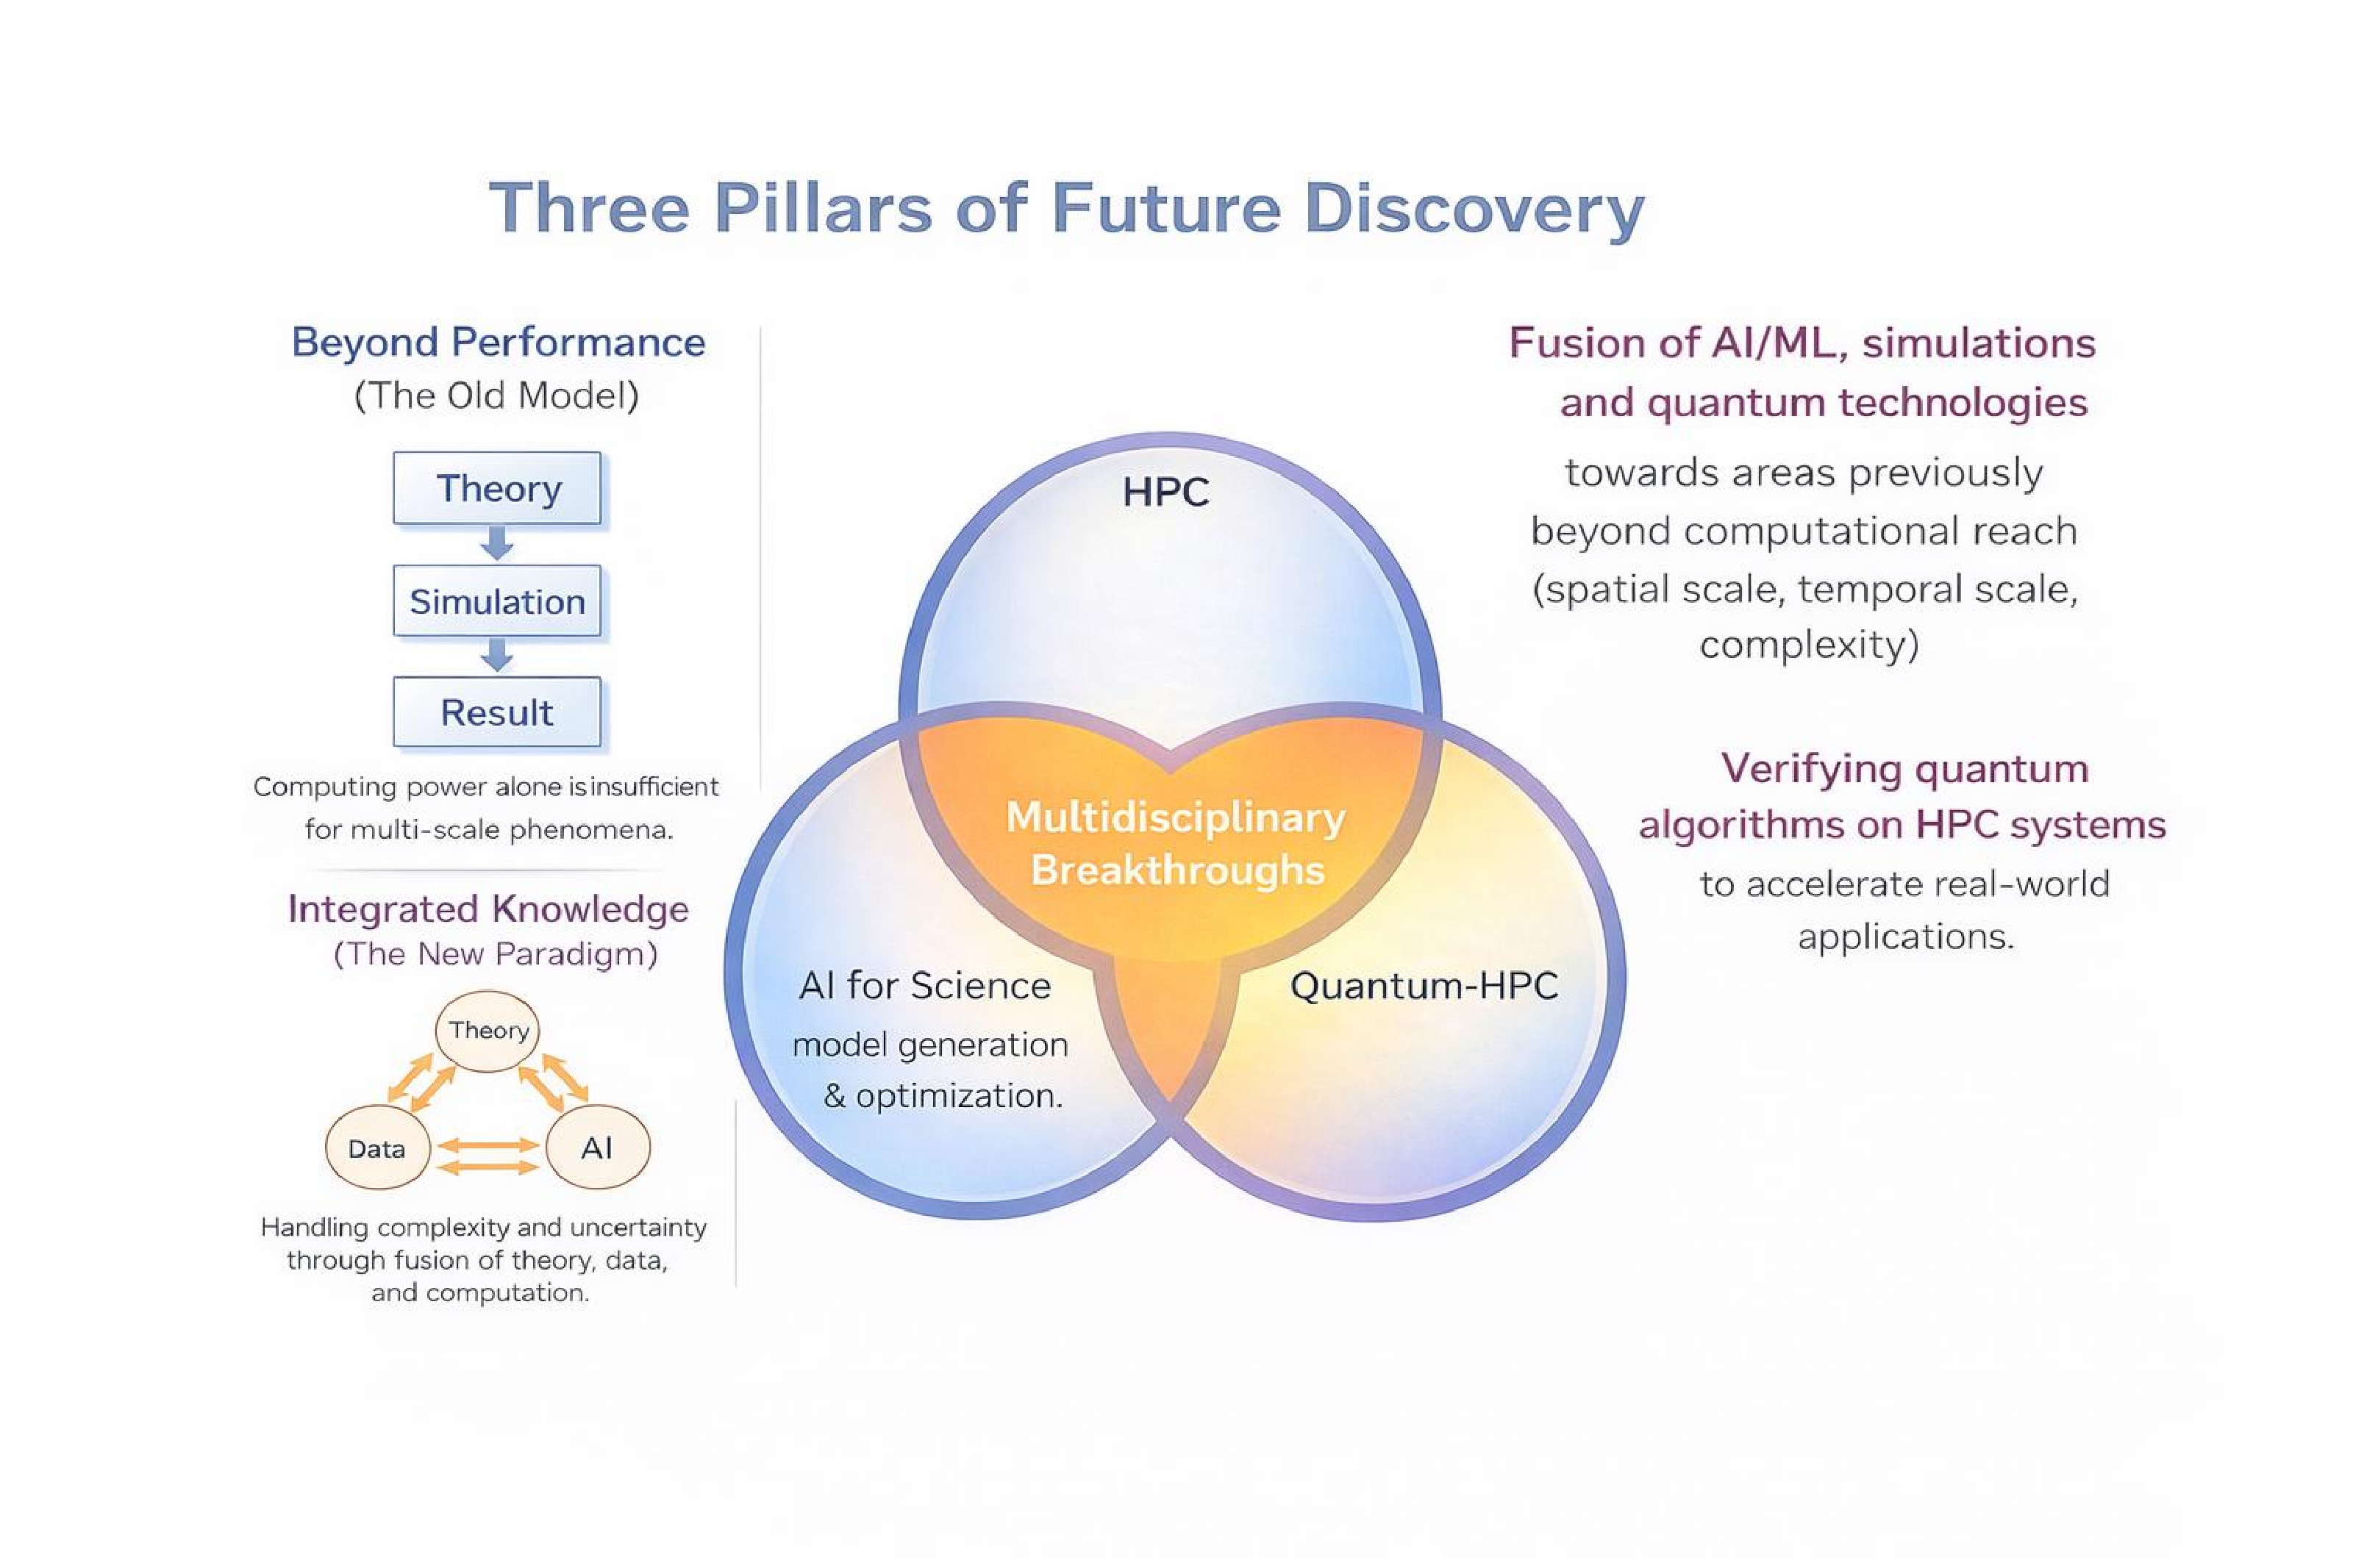
\includegraphics[width=0.9\linewidth]{Futurevision.pdf}};
    \end{tikzpicture}
  \end{center}

\end{frame}

%==============================================================================
\section{Case Studies}
%==============================================================================

\begin{frame}{Case Studies — Overview}

  \begin{columns}[T]
    \begin{column}{0.48\textwidth}
      \begin{block}{Quantum Control}
        RL and neural-network optimisation discover control strategies
        that \emph{outperform} traditional approaches for quantum
        computers and sensors
      \end{block}
      \medskip
      \begin{block}{Quantum Simulation of Many-Body Systems}
        Classical approaches face \emph{exponential} complexity for
        strongly correlated systems; hybrid quantum-classical methods
        may provide new tools
      \end{block}
      \medskip
      \begin{block}{AI-Assisted Hardware Development}
        ML analyses experimental data, identifies noise sources, and
        optimises device architectures — accelerating the path to
        fault-tolerant quantum computers
      \end{block}
    \end{column}
    \begin{column}{0.48\textwidth}
      \begin{block}{Quantum ML for Finance}
        \begin{itemize}
          \item Portfolio optimisation via QAOA / quantum annealing
          \item Quantum kernel methods for financial time series
          \item Quantum generative models for risk analysis and
                Monte-Carlo-style simulations
        \end{itemize}
      \end{block}
      \medskip
      \begin{block}{Applications to Neuroscience}
        \begin{itemize}
          \item QML for high-dimensional neural data representation
          \item Quantum simulation of spin-model-like neural dynamics
        \end{itemize}
      \end{block}
    \end{column}
  \end{columns}

\end{frame}

%------------------------------------------------------------------------------
\begin{frame}{Spotlight: Quantum Control with Reinforcement Learning}

  \begin{columns}[T]
    \begin{column}{0.52\textwidth}
      \textbf{Why is control hard?}
      \begin{itemize}
        \item Parameter spaces of quantum devices are extremely large
        \item Traditional optimisation methods scale poorly
        \item Noise and decoherence degrade any imperfect protocol
      \end{itemize}
      \bigskip
      \textbf{What RL offers:}
      \begin{itemize}
        \item Model-free exploration of huge control landscapes
        \item Discovers non-intuitive protocols
        \item Adapts online to hardware drift
      \end{itemize}
    \end{column}
    \begin{column}{0.44\textwidth}
      \begin{block}{Key References}
        \footnotesize
        \begin{itemize}
          \item Bukov \& Marquardt,
                \emph{RL for Quantum Technology},
                arXiv:2601.18953 (2026)
          \item Belliardo et al.,
                \emph{Model-aware RL for Bayesian quantum metrology},
                Quantum \textbf{8}, 1555 (2024)
        \end{itemize}
      \end{block}
      \medskip
      \small
      \textcolor{mqblue}{Result:} RL agents have demonstrated gate
      fidelities competitive with hand-tuned protocols on real hardware.
    \end{column}
  \end{columns}

\end{frame}

%------------------------------------------------------------------------------
\begin{frame}{Spotlight: Quantum ML for Finance and Neuroscience}

  \begin{columns}[T]
    \begin{column}{0.48\textwidth}
      \textbf{Finance}
      \begin{itemize}
        \item Large datasets, stochastic dynamics,
              high-dimensional optimisation
        \item \textbf{QAOA} / quantum annealing for combinatorial
              portfolio optimisation
        \item \textbf{Quantum kernel methods} — data encoded in
              quantum states; similarity evaluated in Hilbert space
        \item \textbf{Quantum generative models} — variational circuits
              or quantum Boltzmann machines for risk analysis
      \end{itemize}
    \end{column}
    \begin{column}{0.48\textwidth}
      \textbf{Neuroscience}
      \begin{itemize}
        \item Brain: billions of interacting neurons, highly complex
              dynamical system
        \item ML already central for analysing neural recordings
        \item \textbf{QML} may represent high-dimensional neural data
              or model complex probability distributions
        \item Models of collective neural behaviour resemble
              \textbf{spin systems} from statistical physics
              $\Rightarrow$ methods from quantum many-body physics
              may offer new insights
      \end{itemize}
    \end{column}
  \end{columns}

\end{frame}

%==============================================================================
\section{Future Strategies}
%==============================================================================

\begin{frame}{Future Strategies and Requirements}

  \begin{columns}[T]
    \begin{column}{0.32\textwidth}
      \begin{block}{\centering Interdisciplinary\\Collaboration}
        \centering\medskip
        Physics $\;\cdot\;$ Computer science $\;\cdot\;$
        Mathematics $\;\cdot\;$ Engineering
        \medskip

        \small Key challenges lie \emph{at the intersection}
        of these fields
      \end{block}
    \end{column}
    \begin{column}{0.32\textwidth}
      \begin{block}{\centering Education \&\\Training}
        \centering\medskip
        Future researchers need expertise in:
        \medskip

        \small Physics $\;\cdot\;$ Numerical methods $\;\cdot\;$
        Machine learning $\;\cdot\;$ Quantum information science
      \end{block}
    \end{column}
    \begin{column}{0.32\textwidth}
      \begin{block}{\centering Research\\Infrastructure}
        \centering\medskip
        Integrated platforms combining:
        \medskip

        \small HPC resources $\;\cdot\;$ Experimental quantum platforms $\;\cdot\;$
        ML-driven analysis environments
      \end{block}
    \end{column}
  \end{columns}

  \bigskip
  \begin{center}
    \textcolor{mqblue}{\bfseries
    Realising this potential requires coordinated efforts across
    multiple disciplines — no single community can do it alone.}
  \end{center}

\end{frame}

%==============================================================================
\section{Conclusions}
%==============================================================================

\begin{frame}{Conclusions}

  \begin{itemize}
    \setlength\itemsep{8pt}
    \item AI and quantum technologies are \textbf{rapidly reshaping}
          the landscape of computational science
    \medskip
    \item Their mutual interaction, combined with advances in HPC,
          is transforming how scientific problems are approached and solved
    \medskip
    \item The integration of \textbf{theory, simulation, machine learning,
          and quantum hardware} may enable entirely new forms of
          scientific discovery
    \medskip
    \item Promising near-term applications span:
          quantum control, many-body simulation, hardware development,
          finance, and neuroscience
  \end{itemize}

  \bigskip
  \begin{center}
    \begin{beamercolorbox}[rounded=true,sep=6pt,center,wd=0.88\linewidth]{block title}
      As these technologies continue to mature, their convergence
      will play a central role in addressing some of the most
      challenging problems in physics, chemistry, and materials science.
    \end{beamercolorbox}
  \end{center}

\end{frame}

%------------------------------------------------------------------------------
\begin{frame}{Key References}

  \footnotesize
  \begin{thebibliography}{5}

    \bibitem{goodfellow2016}
    I.~Goodfellow, Y.~Bengio, and A.~Courville,
    \emph{Deep Learning},
    MIT Press (2016).

    \bibitem{preskill2018}
    J.~Preskill,
    Quantum computing in the NISQ era,
    \emph{Quantum} \textbf{2}, 79 (2018).

    \bibitem{bukov2026}
    M.~Bukov and F.~Marquardt,
    Reinforcement learning for Quantum Technology,
    arXiv:2601.18953 (2026).

    \bibitem{belliardo2024}
    F.~Belliardo, F.~Zoratti, F.~Marquardt, and V.~Giovannetti,
    Model-aware reinforcement learning for high-performance
    Bayesian experimental design in quantum metrology,
    \emph{Quantum} \textbf{8}, 1555 (2024).

    \bibitem{schuld2021}
    M.~Schuld and F.~Petruccione,
    \emph{Machine Learning with Quantum Computers},
    Springer-Verlag (2021).

  \end{thebibliography}

\end{frame}


\end{document}

